\documentclass[11pt]{article}
\usepackage{times}
\pagestyle{empty}
\parindent 0px
\usepackage{geometry}
 \geometry{
 a4paper,
 total={170mm,257mm},
 left=20mm,
 top=20mm,
 }
 
\title{CS5691: Assignment 3}
\author{Akshat Meena (CS19B052) \\ Shubham Patel (ME19B170)}
\date{}
\usepackage{graphicx}
\graphicspath{ {../../Plots/K-Means/Synthetic Data}{../../Plots/K-Means/Image Data} }

\begin{document}
\maketitle

\begin{center}
\begin{Large}
A. K-means, GMM
\end{Large}
\end{center}

\begin{enumerate}
	\begin{large}
	\item \textbf{Synthetic Dataset}
	\end{large}
	
	\begin{itemize}
		\item First we do the observations for different number of clusters (K=2,4,8,16) for both diagonal and non diagonal covariance matrices.
		\item We start with plotting the GMMs for K=2, we observe that there is not much difference in the decision surface for both the covariance matrices. For Diagonal matrix it is a little smoother.
	\begin{figure}[h]
		\caption{
		\begin{small}
		GMMs for synthetic data for K = 2 and Non-Diagonal and Diagonal Covariance for each class
		\end{small}
		}
		\centering
		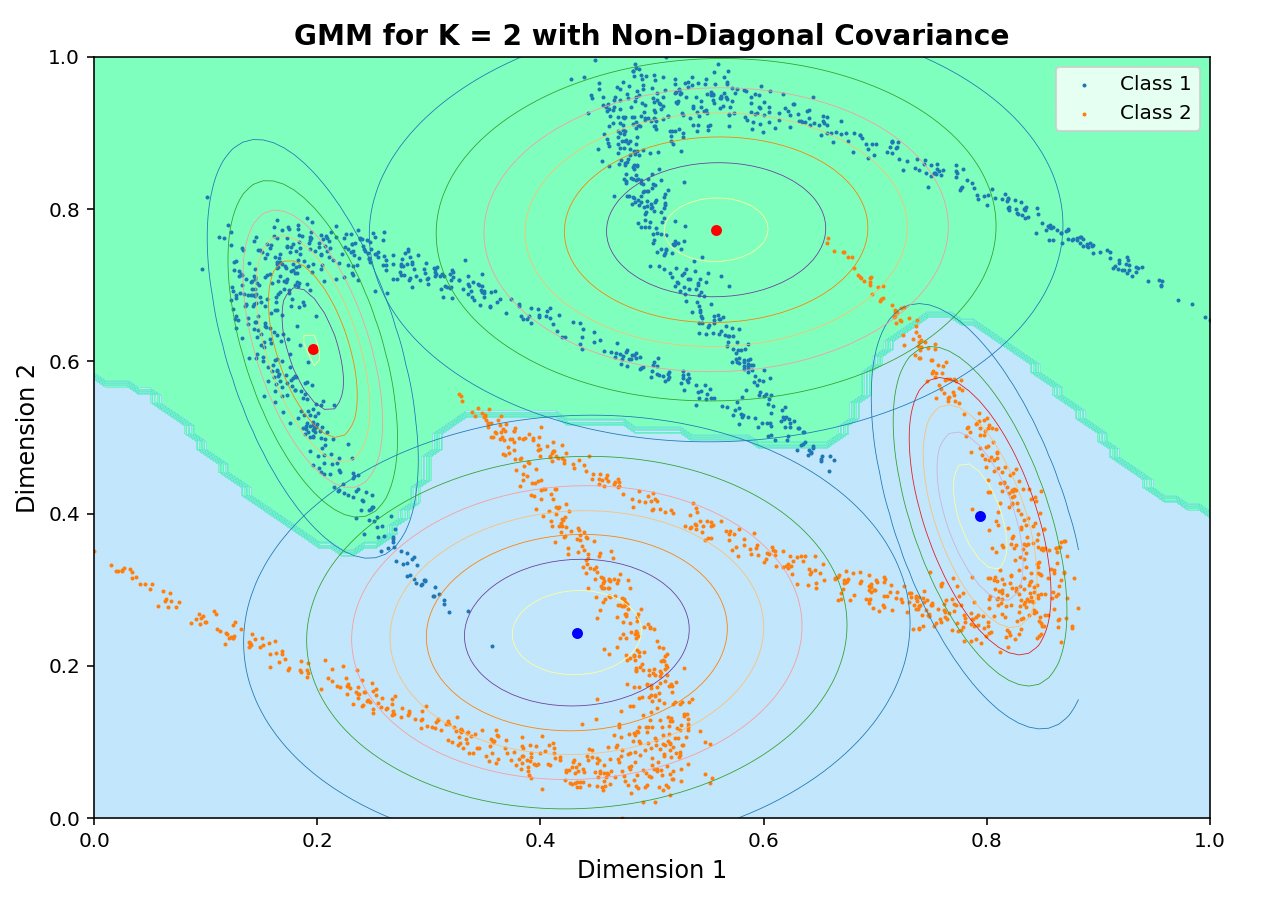
\includegraphics[scale=0.35]{K2_ND}
		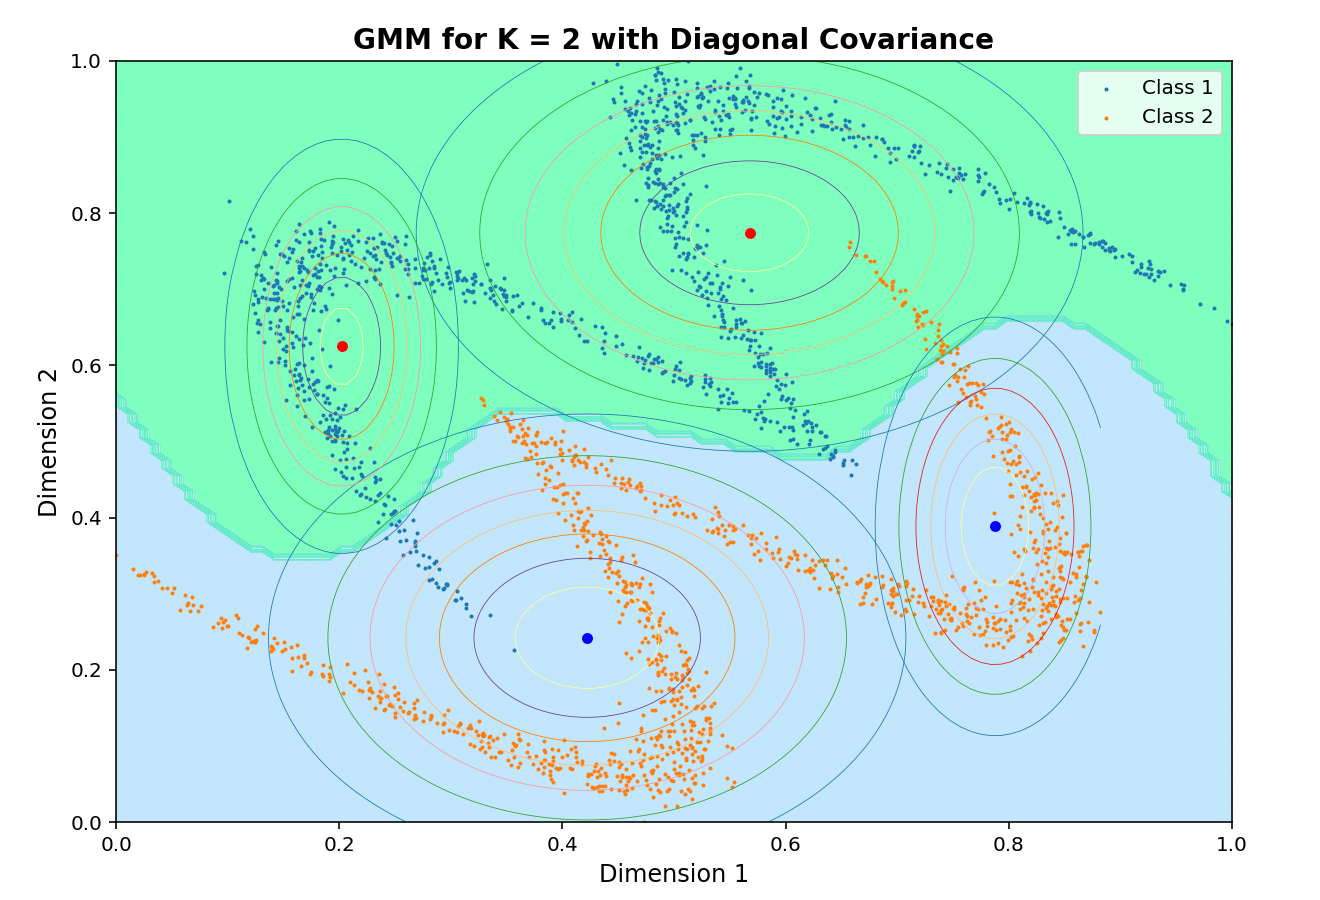
\includegraphics[scale=0.35]{K2_D}
	\end{figure}\\
	
	\item Next we plot for K = 4. We observe that the decision plot for diagonal covariance matrix is better than non-diagonal.
	\item We observe that the decision surface starts taking better shape.
	\begin{figure}[h]
		\caption{
		\begin{small}
		GMMs for synthetic data for K = 4 and Non-Diagonal and Diagonal Covariance for each class
		\end{small}
		}
		\centering
		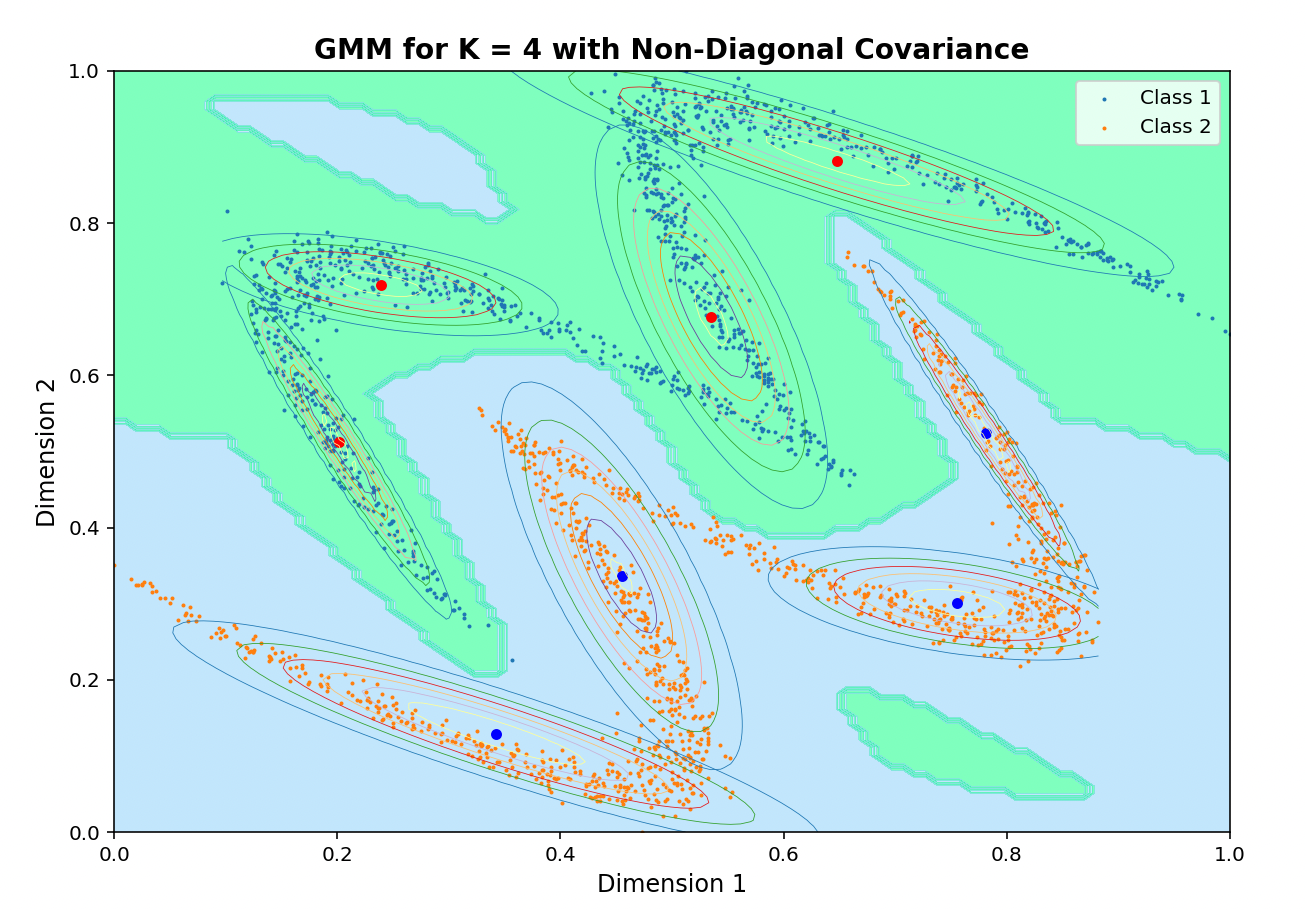
\includegraphics[scale=0.35]{K4_ND}
		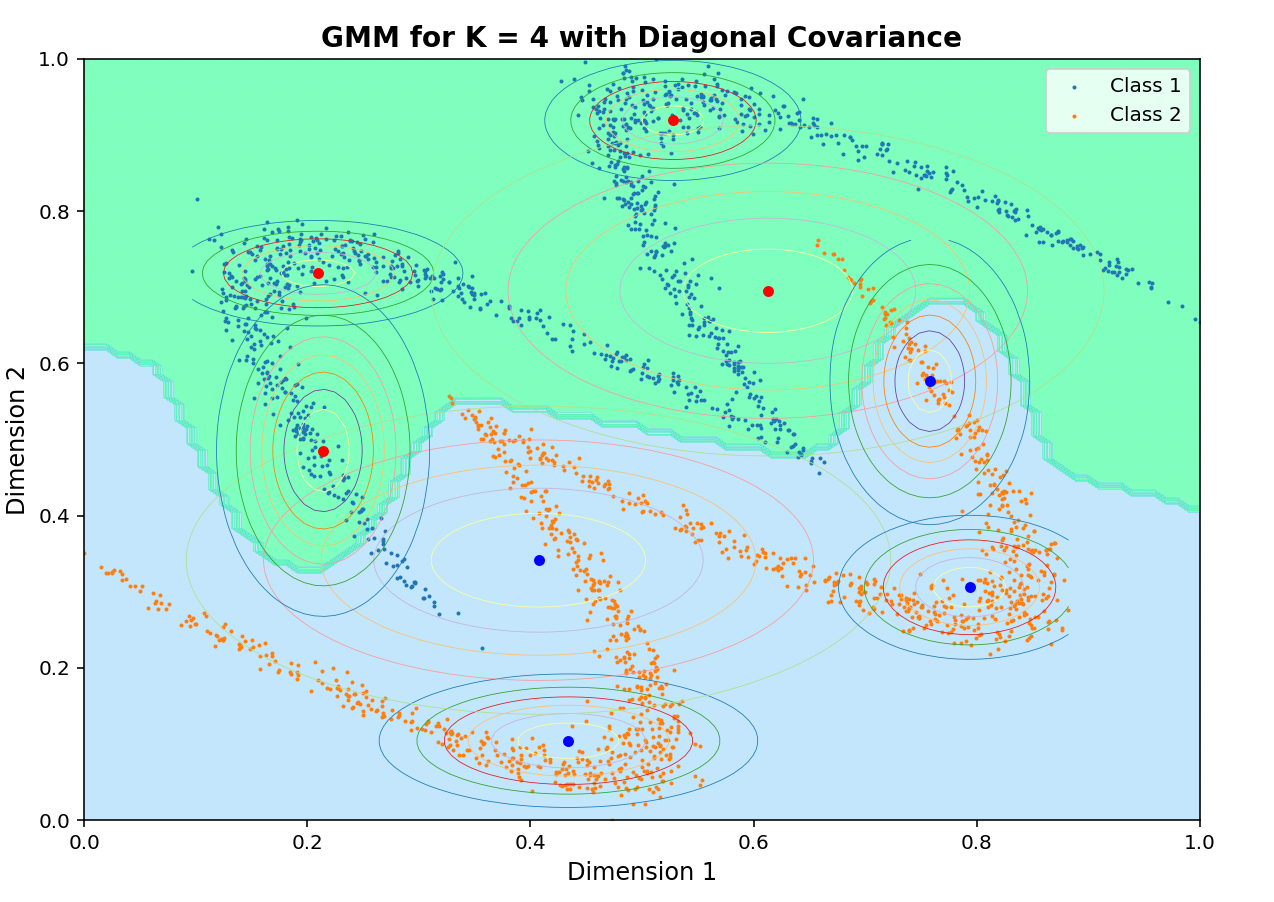
\includegraphics[scale=0.35]{K4_D}
	\end{figure}\\
	\pagebreak
	\item For K = 8, we see the contour of the Gaussian fitting each branch in the entire model properly. The contours of the branches are aligned with the the branch's alignment and each branch completely fit in case of non-diagonal covariance matrix
	\begin{figure}[h]
		\caption{
		\begin{small}
		GMMs for synthetic data for K = 8 and Non-Diagonal and Diagonal Covariance for each class
		\end{small}
		}
		\centering
		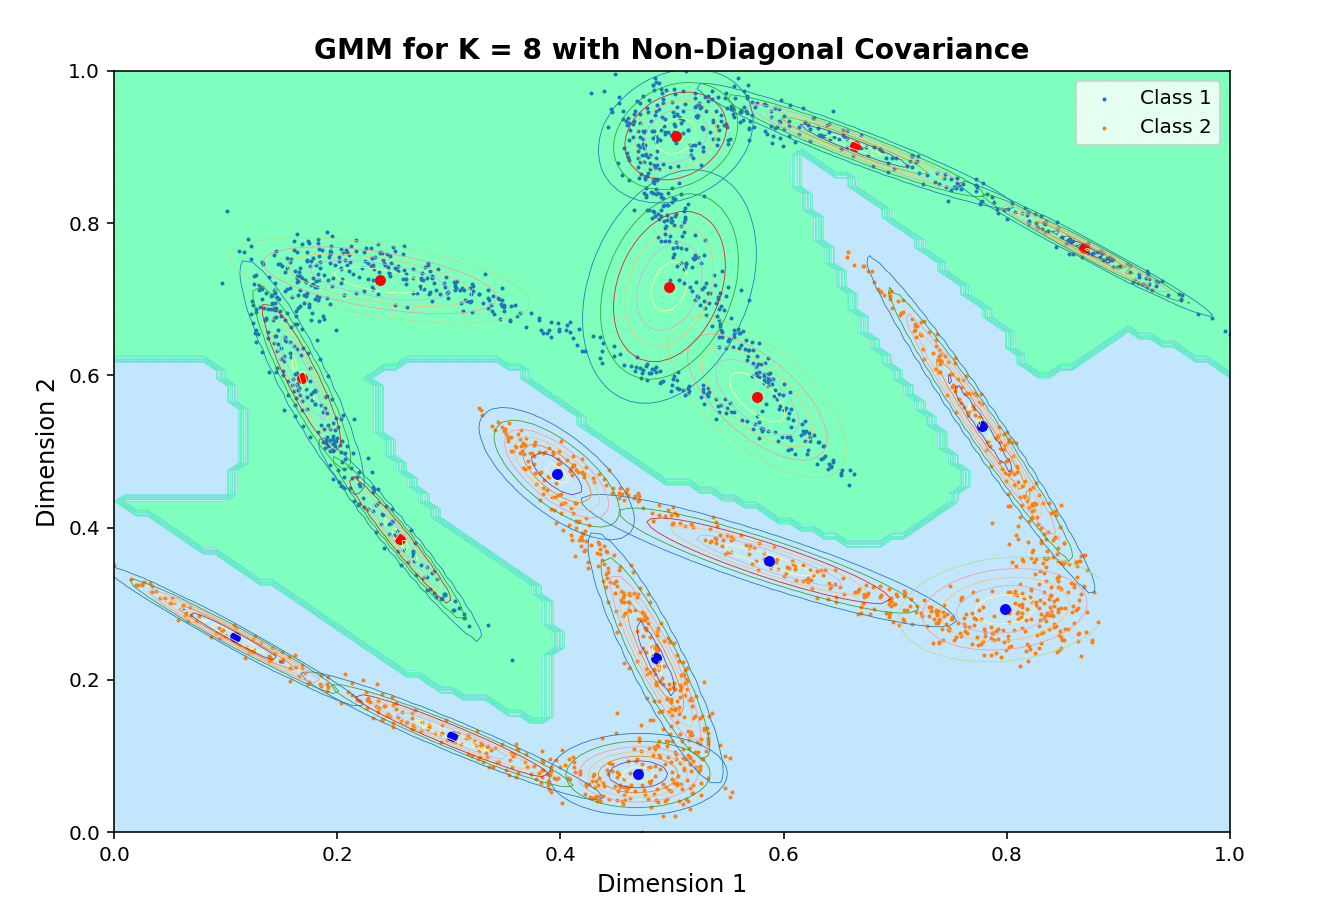
\includegraphics[scale=0.3]{K8_ND}
		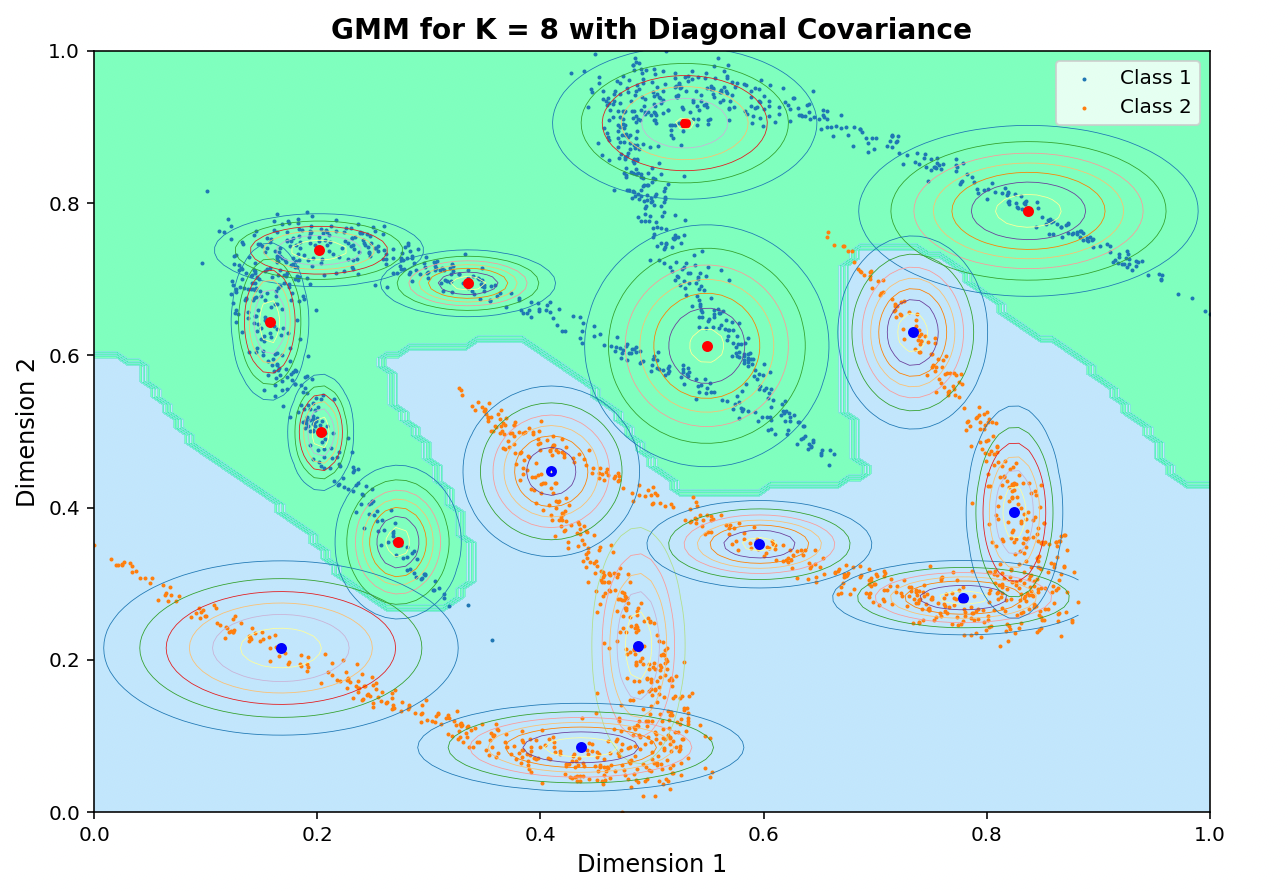
\includegraphics[scale=0.3]{K8_D}
	\end{figure}\\
	
	\item When we choose K = 16, we see that the data starts getting overfitted, more in case of non-diagonal covariance matrix. We also see that the decision surface does very exact classification.
	\begin{figure}[h]
		\caption{
		\begin{small}
		GMMs for synthetic data for K = 16 and Non-Diagonal and Diagonal Covariance for each class
		\end{small}
		}
		\centering
		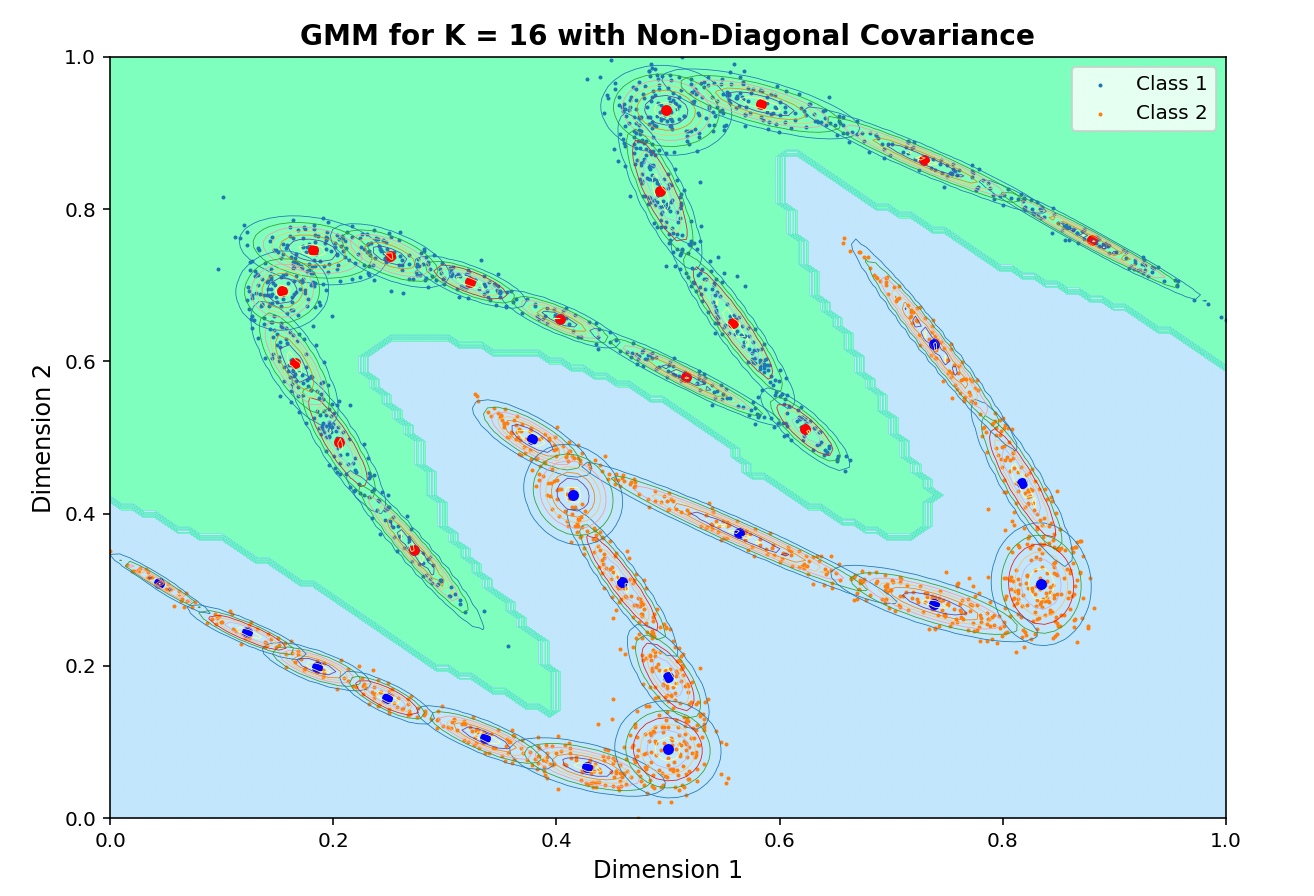
\includegraphics[scale=0.3]{K16_ND}
		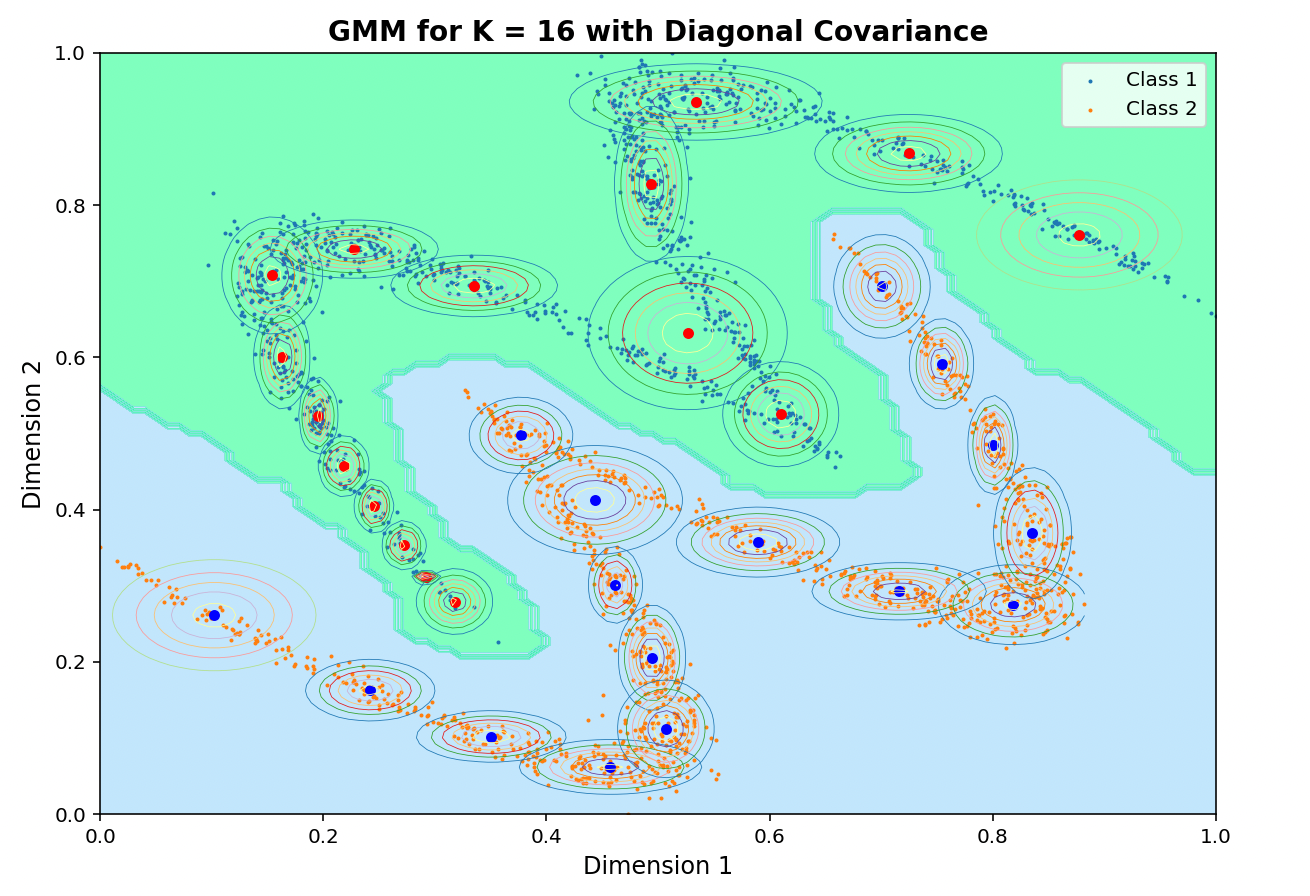
\includegraphics[scale=0.3]{K16_D}
	\end{figure}\\
	\item \textbf{ROC Curve}
	\begin{figure}[h]
		\caption{
		\begin{small}
		ROC Curve for Synthetic Data
		\end{small}
		}
		\centering
		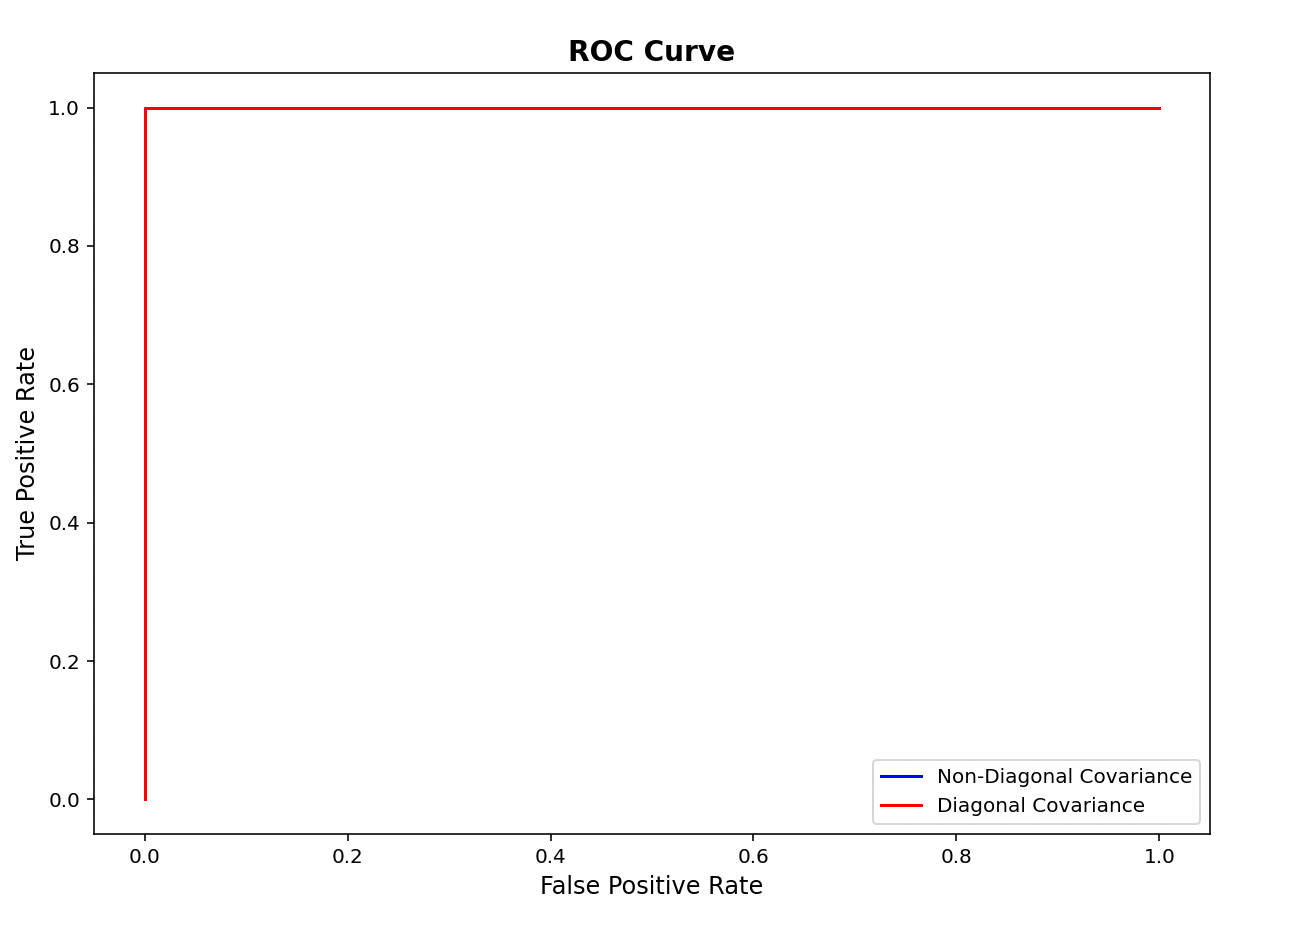
\includegraphics[scale=0.4]{ROC}
	\end{figure}\\
	\pagebreak
	\item \textbf{DET Curve}
	\begin{figure}[h]
		\caption{
		\begin{small}
		DET Curve for Synthetic Data
		\end{small}
		}
		\centering
		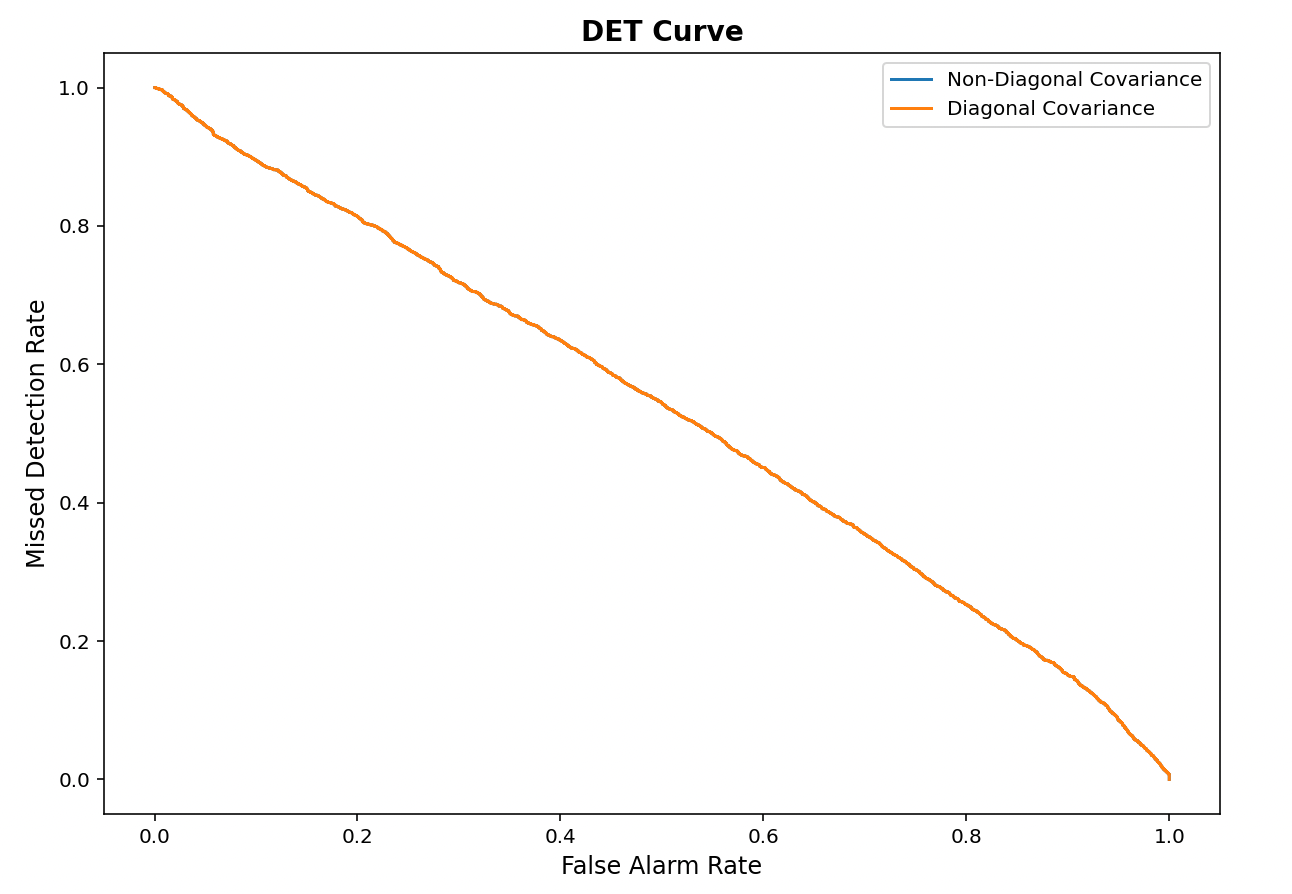
\includegraphics[scale=0.5]{DET}
	\end{figure}\\
	\item \textbf{Confusion Matrix}
	\begin{figure}[h]
		\caption{
		\begin{small}
		Confusion Matrix for both Non Diagonal and Diagonal Matrix and K = 16
		\end{small}
		}
		\centering
		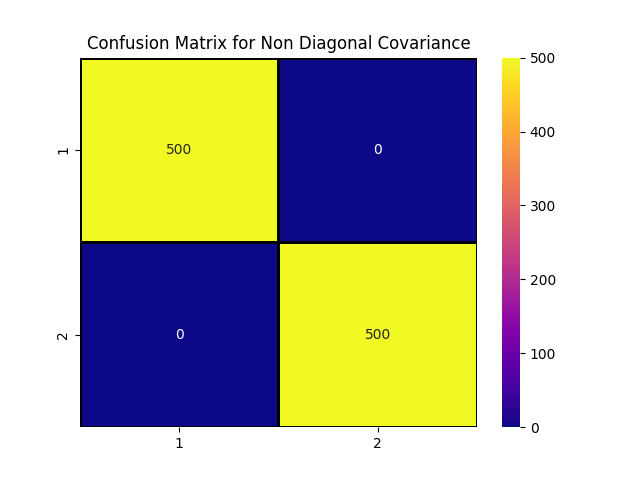
\includegraphics[scale=0.52]{CM_ND}
		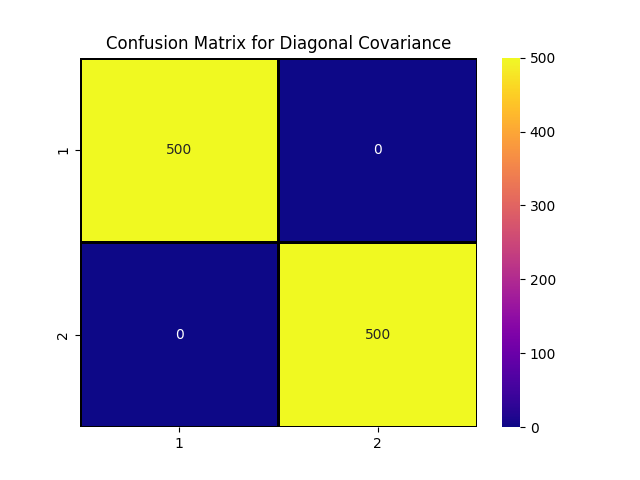
\includegraphics[scale=0.52]{CM_D}
	\end{figure}\\
	\end{itemize}
	\pagebreak
	\begin{large}
	\item \textbf{Image Dataset}
	\end{large}
	
	\begin{itemize}
		\item For Diagonal Covariance Matrix we get accuracy of \textbf{37.64\%}
	\begin{figure}[h]
	\caption{
	\begin{small}
	Confusion Matrix for K = 4 and 10 iterations for Diagonal Covariance
	\end{small}
	}
	\centering
	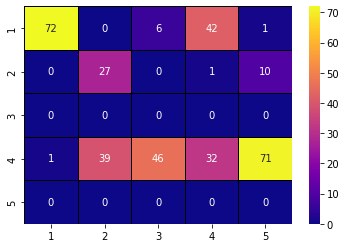
\includegraphics[scale=1]{K4_10_1}
	\end{figure}\\
	\item We observe that classification is better with diagonal covariance than non diagonal
	\end{itemize}
\end{enumerate}

\end{document}